\documentclass{llncs}

\pagestyle{plain}

\usepackage[english]{babel}
\usepackage{graphicx}
\usepackage{listings}
\usepackage{times}
\usepackage{color}
\usepackage{xspace}
\usepackage{booktabs}
\usepackage{subfigure}
\usepackage[hyphens]{url}
\usepackage{wrapfig}
\usepackage{psharp}

\urlstyle{rm}

%\newcommand{\TODO}[1]{\textcolor{red}{\textbf{TODO:} #1}}
%\newcommand{\PDComment}[1]{\textcolor{cyan}{\textbf{PD:} #1}}

% General macros
\newcommand{\ps}{P\#\xspace}
\newcommand{\cs}{C\#\xspace}

\newcommand{\newparagraph}[1]{\smallskip\noindent\textbf{#1 }}

\begin{document}

\title{Getting Started with \ps}

\author{Pantazis Deligiannis$^1$, Akash Lal$^2$, Shaz Qadeer$^3$}
\institute{$^1$ \textsf{p.deligiannis@imperial.ac.uk}, \emph{Imperial College London}, UK\\$^2$ \textsf{akashl@microsoft.com}, \emph{Microsoft Research}, India\\$^3$ \textsf{qadeer@microsoft.com}, \emph{Microsoft Research}, USA}

\maketitle

\section{Introduction}
\label{sec:intro}

\ps~\cite{pd2015psharp} is an extension of the \cs language, designed to significantly ease the process of developing and testing asynchronous applications in Microsoft's .NET platform. To achieve this goal, \ps has the following core capabilities:

\begin{itemize}
\item Exposes a computational model based on \emph{communicating state-machines} (similar concept to actors from other asynchronous programming languages). \ps machines are built on top of the Task Parallel Library (TPL) and communicate by explicitly \emph{sending} and implicitly \emph{receiving events}, an approach commonly used in building web services and distributed systems. Because \ps \emph{fully interoperates} with \cs, the \ps programmer can easily blend \ps and \cs code, which makes it \emph{easy to integrate} with existing .NET projects.

\item Provides powerful mechanisms for writing \emph{concurrency unit tests} of \ps applications, as well as legacy \cs code that uses message-passing. When executing a concurrency unit test, the \ps runtime is invoked in \emph{systematic testing} mode, where it takes control of the underlying task scheduler and systematically explores \emph{event handler interleavings} to find bugs, such as safety and liveness property violations, and runtime exceptions.

\item Enables the developer to specify \emph{models} of the application's \emph{environment} (e.g. the client, a sub-module of a distributed system or the network). These models can introduce non-deterministic choices (e.g. to model node failures) that are captured by the \ps runtime and/or abstract away implementation details of the real system that are irrelevant to the properties being checked. When systematically testing a \ps application, these models \emph{substitute} the real environment. This can be effectively used for \emph{compositional} (and thus scalable) testing of large systems.
\end{itemize}

\newparagraph{Programming model} \ps is built on top of the Roslyn\footnote{\url{https://github.com/dotnet/roslyn}} compiler and provides new language primitives (which are largely based on Microsoft's P~\cite{desai2013p} programming language) for creating machines, sending events from one machine to another, and writing assertions about system properties. Each machine has an input queue, states, state transitions, event handlers, fields and methods. Machines run concurrently with each other, each executing an event handling loop that dequeues an event from the input queue and handles it by executing a sequence of operations. Each operation might update a field, create a new machine, or send an event to another machine. In \ps, create machine operations and send operations are non-blocking. In the case of a send operation the message is simply enqueued into the input queue of the target machine.\\

\newparagraph{Usage} There are many different ways that someone can use \ps to create highly-reliable asynchronous .NET applications:

\begin{itemize}
\item Use the \emph{surface syntax} of \ps to write an entire application from scratch. The surface syntax directly extends \cs with new language constructs, which allows for rapid prototyping. The main disadvantage of this approach is that \ps does not yet fully integrate with the Visual Studio integrated development environment (IDE), and thus does not support high-productivity features such as IntelliSense (e.g. for auto-completition and automated refactoring).

\item Use \ps as a \cs library to write an entire application from scratch. This approach is more verbose than the above, but allows full integration with Visual Studio. Note that most examples in this guide will use the \ps surface syntax as it is less verbose. See Section~\ref{} for an example of using \ps as a \cs library.

\item Mix \ps projects with \cs projects. \ps compiles to \cs using Roslyn, which allows easy integration of the two languages in the same solution.

\item Use \ps only for modeling the environment of a legacy \cs system and then systematically test it. Note that the assumption is that the \cs code that will be tested is sequential and deterministic. If not, bugs might still be found, but the \ps runtime cannot fully control the underlying scheduler and, thus, loses efficiency.
\end{itemize}

\newparagraph{Repository} The \ps language is publicly available as open-source and can be found at its git repository at \textbf{\url{https://github.com/p-org/PSharp}}.\\

\noindent
In the rest of this guide, we first introduce basic features of a \ps program (Section~\ref{sec:basics}) and then discuss how \ps can be embedded in \cs code (Section~\ref{sec:ps2cs}). Next, we present an example of a simple program using both the \ps surface syntax and \ps as a library (Section~\ref{sec:simple}). We then present the more advanced features of \ps (Section~\ref{sec:advanced}). Next, we illustrate how someone can write safety properties in \ps (see Section~\ref{sec:safetyproperties}), which can be systematically checked for bugs. Finally, we provide an overview of the tools for compiling and systematically testing a \ps program and conclude with a glossary of all \ps-specific features in our language.


\section{Basic features of a \ps program}
\label{sec:basics}

A \ps program is a collection of \inlinepsharp{event} and \inlinepsharp{machine} declarations and, optionally, other top-level \cs declarations, such as \inlinepsharp{class} and \inlinepsharp{struct}. All top-level declarations must be declared inside a \inlinepsharp{namespace}, as in \cs. If someone uses the \ps high-level syntax, then events and machines must be declared inside a \texttt{.psharp} file, while \cs top-level declarations must be declared in a \texttt{.cs} file. On the other hand, if someone uses \ps as a \cs library, all the code must be written inside a \texttt{.cs} file.

State machines are first-class citizens of the \ps language and can be declared in the following way:

\begin{psharpNoLines}
machine Server { ... }
\end{psharpNoLines}

\noindent
This declares a machine named \inlinepsharp{Server}. Machine declarations are very similar to class declarations in \cs and can contain fields, states and methods. Fields can be declared similar to how fields are declared in \cs:

\begin{psharpNoLines}
machine Server {
  machine client;
}
\end{psharpNoLines}

\noindent
This declares a field named \inlinepsharp{client} of type \inlinepsharp{machine}, which contains the \emph{unique id} of a dynamically-created \ps machine. This id can be used to send an event to \inlinepsharp{client}, as discussed later in the guide. Fields in \ps can have an arbitrary type; all \cs types, as well as user-defined types, are allowed. Note that the fields of a machine \emph{cannot} be \inlinepsharp{public} or \inlinepsharp{internal}; they can only be accessed from the local scope of an instance of a machine. If a user declares a field as \inlinepsharp{public} or \inlinepsharp{internal}, then the compiler will exit with an appropriate error.

Machine states can be declared as follows:

\begin{psharpNoLines}
machine Server {
  machine client;
  start state Init { ... }
  state Active { ... }
}
\end{psharpNoLines}

\noindent
This declares two states in the \inlinepsharp{Server} machine: \inlinepsharp{Init} and \inlinepsharp{Active}. A machine \emph{must} declare an \emph{initial} state, which will be the first state that the machine will start execution. The \inlinepsharp{start} modifier is used for declaring an initial state. In the above example, the \inlinepsharp{Init} state has been declared as the initial state of the \inlinepsharp{Server} machine.

A \inlinepsharp{state} declaration can optionally contain a number of state-specific declarations, as seen in the following example:

\begin{psharpNoLines}
state SomeState {
  entry { ... }
  exit { ... }
}
\end{psharpNoLines}

\noindent
A code block indicated by \inlinepsharp{entry} \{ ... \} denotes an action that is executed when the state is entered, while a code block indicated by \inlinepsharp{exit} \{ ... \} denotes an action that is executed when the state exits. The \inlinepsharp{entry} and \inlinepsharp{exit} actions are blocks of arbitrary \ps and \cs statements. An example of an \inlinepsharp{entry} action is the following:

\begin{psharpNoLines}
entry {
  this.client = create(Client, this);
  send(this.client, Ping);
  raise(Unit);
}
\end{psharpNoLines}

\noindent
The above action contains three of the most important \ps statements. The \inlinepsharp{create} statement, creates a new instance of the \inlinepsharp{Client} machine and stores the unique id of this instance in the field \inlinepsharp{client}. Next, the \inlinepsharp{send} statement sends an event (in this case the event \inlinepsharp{Ping}) to a target machine (in this case the machine whose address is stored in the field \inlinepsharp{Client}). When an event is sent, it is enqueued in the event queue of the target machine. The target machine can then dequeue the event and handle it concurrently from the sender machine. Finally, The \inlinepsharp{raise} statement sends an event to the caller machine (i.e. sends an event to itself). In \ps, when a machine raises an event, the raised event is not enqueued; the machine terminates execution of the enclosing code block and handles the event immediately.

Events (e.g. \inlinepsharp{Ping} and \inlinepsharp{Unit} in our case) can be simply declared as follows:

\begin{psharpNoLines}
event Ping;
event Unit;
\end{psharpNoLines}

\noindent
A machine can optionally send data to another machine, either when creating a new machine (via the \inlinepsharp{create} statement) or when sending an event to a machine (via the \inlinepsharp{send} statement). A machine can also send data to itself (e.g. for processing in a later state) via the \inlinepsharp{raise} statement. In the previous example, the machine sends \inlinepsharp{this} to \inlinepsharp{client}. By default, \inlinepsharp{this} denotes a reference to the instance of the machine that uses it, but when sending \inlinepsharp{this} to another machine, it sends the unique id of the machine (e.g. so the other machine can use it to send something back). The receiver machine (in our case \inlinepsharp{client} can retrieve the sent data by using the keyword \inlinepsharp{payload} and casting it to its expected type; in this case the \inlinepsharp{payload} has to be casted to the \inlinepsharp{machine} type (as it is the id of the sender machine).

As discussed earlier, the \inlinepsharp{create} and \inlinepsharp{send} statements are non-blocking. The \ps runtime will take care of all the underlying asynchrony, and thus the user does not need to create and manage explicit tasks. For efficiency, the \ps runtime executes the event handler on the context of a separate TPL task instead of a more heavyweight thread.

Other than the \inlinepsharp{entry} and \inlinepsharp{exit} declarations, all other declarations inside a state are related to \emph{event-handling}. Two of the most important event-handling declarations in \ps are the following:

\begin{psharpNoLines}
state SomeState {
  on Unit goto AnotherState;
  on Pong do SomeAction;
}
\end{psharpNoLines}

\noindent
The declaration \inlinepsharp{on Unit goto AnotherState} indicates that when the machine receives the \inlinepsharp{Unit} event in \inlinepsharp{SomeState}, it must handle the event by exiting the
state and transitioning to \inlinepsharp{AnotherState}. The declaration \inlinepsharp{on Pong do SomeAction} indicates that the \inlinepsharp{Pong} event must be handled by invoking the action \inlinepsharp{SomeAction}. Each event can be associated with at most one handler in a particular state of a machine.

Actions in \ps are methods with no parameters. A \ps method (declared exactly like a typical \cs method) can contain arbitrary \ps and \cs statements. Note that the methods of a machine \emph{cannot} be \inlinepsharp{public} or \inlinepsharp{internal} (similar to machine fields). If a user declares a method as \inlinepsharp{public} or \inlinepsharp{internal}, then the compiler will exit with an appropriate error. \ps also supports \emph{anonymous} actions. For example, the declaration \inlinepsharp{on Pong do} \{ ... \} is such an anonymous action, which states that the block of statements between the braces must be executed when event \inlinepsharp{Pong} is dequeued.\\


\section{Embedding \ps into \cs}
\label{sec:ps2cs}

Interoperability between the two languages is in the heart of the \ps programming approach. This is because \ps is essentially \cs, but with some extra key features for enabling safer and easier-to-test asynchronous .NET programming. Even to start executing a \ps program, the programmer has to create the very first machine from inside the context of a \cs method. This can be done by calling the \inlinepsharp{CreateMachine} method (provided by the \inlinepsharp{PSharpRuntime} APIs) from any \cs method (typically the \inlinepsharp{Main} method) as follows:

\begin{psharpNoLines}
public class Program {
  static void Main(string[] args) {
    PSharpRuntime.CreateMachine(typeof(Server));
    Console.ReadLine();
  }
}
\end{psharpNoLines}

\noindent
The \inlinepsharp{CreateMachine} method accepts as an argument the type of the machine to be created (in our case \inlinepsharp{Server}) and an optional payload (not used in this example). Because \inlinepsharp{CreateMachine} is non-blocking, we use the \inlinepsharp{Console.ReadLine()} statement so that the program does not exit prematurely.

The \inlinepsharp{PSharpRuntime} APIs also provide the \inlinepsharp{SendEvent} method for enqueueing events to a \ps machine from \cs code (also not used in this example). This method accepts as an argument a \inlinepsharp{MachineId} object (which corresponds to the unique id of a machine), an event and an optional payload. The \inlinepsharp{MachineId} object is returned when creating a machine via the \inlinepsharp{CreateMachine} method.

Although the programmer has to use the above methods to send data from \cs code to a \ps machine, the opposite is much more straightforward. A typical way to achieve this is to pass a reference to a \cs object as a payload to a \ps machine, and then invoke a method (or access a field) on that object.


\section{A simple \ps program}
\label{sec:simple}

The following example contains a \inlinepsharp{Server} machine and a \inlinepsharp{Client} machine communicating with each other via sending and receiving \inlinepsharp{Ping} and \inlinepsharp{Pong} events.\\

\begin{psharp}[caption=Simple PingPong application written in the \ps high-level syntax., label=fig:simple_example_ps]
// PingPong.psharp
namespace PingPong {
  event Ping;
  event Pong;
  event Unit;
  
  machine Server {
    machine client;

    start state Init {
      entry {
        this.client = create(Client, this);
        raise(Unit);
      }
      on Unit goto Active;
    }

    state Active {
      entry {
        SendPing();
      }
      on Pong do SendPing;
    }

    void SendPing() {
      send(this.client, Ping);
    }
  }

  machine Client {
    machine server;

    start state Init {
      entry {
        this.server = (machine)payload;
        raise(Unit);
      }
      on Unit goto Active;
    }

    state Active {
      on Ping do {
        send(this.server, Pong);
      };
    }
  }
  
  public class Program {
    static void Main(string[] args) {
      PSharpRuntime.CreateMachine(typeof(Server));
      Console.ReadLine();
    }
  }
}
\end{psharp}

In this example, the \ps program starts with a single instance of \inlinepsharp{Server} being created and then entering state \inlinepsharp{Init}. Let us call this instance of the Server machine \emph{server}. Machine \emph{server} then creates an instance of the \inlinepsharp{Client} machine and raises the event \inlinepsharp{Unit} to enter the state \inlinepsharp{Active}. Let us call this instance of the \inlinepsharp{Client} machine \emph{client}. The machine \emph{client} begins execution when \emph{server} is in the state \inlinepsharp{Active}, then \emph{client} also transitions to the state \inlinepsharp{Active} by raising a event \inlinepsharp{Unit}. From this point on, \emph{server} and \emph{client} keep exchanging \inlinepsharp{Ping} and \inlinepsharp{Pong} events (in an infinite loop).

The above example can be written using \ps as a \cs library as follows:

\begin{psharp}[caption=Simple PingPong application written using \ps as a \cs library., label=fig:simple_example_cs]
// PingPong.cs
using System;
using Microsoft.PSharp;

namespace PingPong {
  class Unit : Event { }
  class Ping : Event { }
  class Pong : Event { }
  
  class Server : Machine {
    MachineId Client;
    
    [Start]
    [OnEntry(nameof(InitOnEntry))]
    [OnEventGotoState(typeof(Unit), typeof(Active))]
    class Init : MachineState { }
    
    void InitOnEntry() {
      this.Client = this.CreateMachine(typeof(Client), this);
      this.Raise(new Unit());
    }
    
    [OnEventDoAction(typeof(Pong), nameof(SendPing))]
    class Active : MachineState {
      protected override void OnEntry() {
        (this.Machine as Server).SendPing();
      }
    }
    
    void SendPing() {
      this.Send(this.Client, new Ping());
    }
  }
  
  class Client : Machine {
    MachineId Server;
    
    [Start]
    [OnEventGotoState(typeof(Unit), typeof(Active))]
    class Init : MachineState {
      protected override void OnEntry() {
        (this.Machine as Client).Server = (MachineId)this.Payload;
        this.Raise(new Unit());
      }
    }
    
    [OnEventDoAction(typeof(Ping), nameof(SendPong))]
    class Active : MachineState { }
    
    void SendPong() {
      this.Send(this.Server, new Pong());
    }
  }
  
  public class Program {
    static void Main(string[] args) {
      PSharpRuntime.CreateMachine(typeof(Server));
      Console.ReadLine();
    }
  }
}
\end{psharp}

The programmer can use \ps as a library by importing the \inlinepsharp{Microsoft.PSharp} library. A \ps machine can be declared by creating a \cs \inlinepsharp{class} that inherits from the type \inlinepsharp{Machine} (provided by the \ps library). A state can be declared by creating a \inlinepsharp{class} that inherits from the type \inlinepsharp{MachineState}. This state class must be nested inside a machine class (no other class besides a state can be nested inside a machine class). The start state can be declared using the \inlinepsharp{[Start]} attribute.

A state transition can be declared using the \inlinepsharp{[OnEventGotoState(...)]} attribute, where the first argument of the attribute is the type of the received event and the second argument is the type of the target state. An optional third argument, is a string that denotes the name of the method to be executed after exiting the state and before entering the new state.

An action handler can be declared using the \inlinepsharp{[OnEventDoAction(...)]} attribute, where the first argument of the attribute is the type of the received event and the second argument is the name of the action to be executed.

All \ps statements (e.g. \inlinepsharp{send} and \inlinepsharp{raise}) are exposed as method calls of the \inlinepsharp{Machine} and \inlinepsharp{MachineState} classes.

Note that even when using \ps as a library, the program has to still be compiled using the \ps compiler as the compiler performs some important static checking to find \ps syntax-related errors and rewriting. Moreover a \ps program can only be systematically tested via a special mode of the \ps compiler as discussed in Section~\ref{}.


\section{Advanced features of \ps}
\label{sec:advanced}

The following is a discussion of more advanced features of \ps, such as termination of machines, specifying safety and liveness properties, and modeling the environment.

\subsection{Termination of \ps machines}
\label{sec:termination}

In order to terminate a \ps machine cleanly, it must dequeue a special event named \inlinepsharp{halt}, which is provided by \ps (the user cannot declare it). A \inlinepsharp{halt} event can be raised and/or send to another machine. Termination of a machine due to an unhandled \inlinepsharp{halt} event is valid behavior (the \ps runtime does not report an error). From the point of view of formal operational semantics, a halted machine is fully receptive and consumes any event that is sent to it. The \ps runtime implements this semantics efficiently by cleaning up resources allocated to a halted machine and recording that the machine has halted. An event sent to a halted machine is simply dropped. A halted machine cannot be restarted; it remains halted forever.

\subsection{Writing safety properties}
\label{sec:safety}

The most important safety specification of a \ps program is that every event dequeued by a machine is handled; otherwise, the \ps runtime reports an unhandled event error. The PingPong program satisfies this specification since the \texttt{Server} machine handles the \texttt{Ping} event and the \texttt{Client} machine handles the \texttt{Pong} event in every state where an event dequeue is possible.

\subsection{Writing liveness properties}
\label{sec:liveness}

\subsection{Modeling the environment}
\label{sec:modeling}

The following example illustrates the more advanced features of the \ps language. This program implements a failure detection protocol. A \inlinepsharp{FailureDetector} machine is given a list of machines, each of which represents a daemon running at a node of a distributed system. The \inlinepsharp{FailureDetector} sends each machine in the list a \inlinepsharp{Ping} event and determines whether a machine has failed. A machine has failed if it does not respond with a \inlinepsharp{Pong} event within a certain time period. The \inlinepsharp{FailureDetector} uses an operating system timer to implement the bounded wait for the \inlinepsharp{Pong} event.


 \begin{figure}[t]
 \centering
 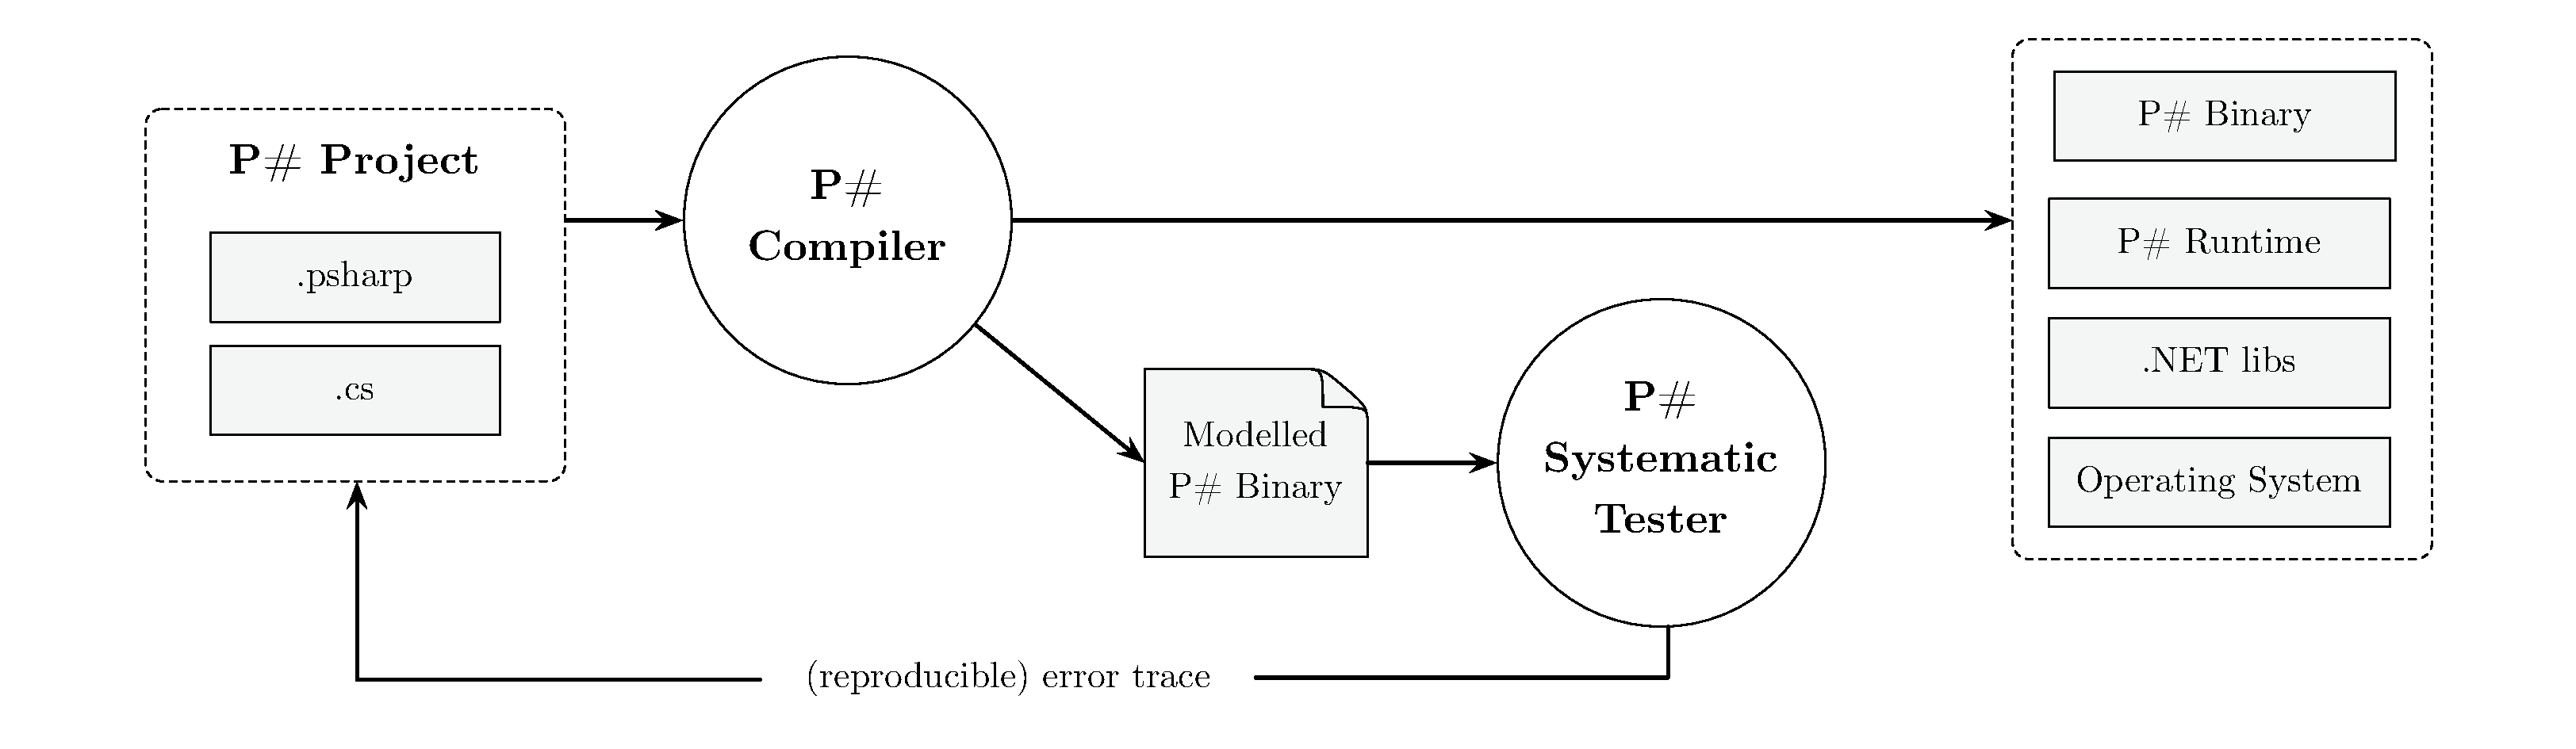
\includegraphics[width=0.95\linewidth]{figures/workflow.pdf}
 \caption{The typical \ps workflow.}
 \label{fig:workflow}
 \end{figure}

%\newpage

\bibliographystyle{plain}
\bibliography{references}

\end{document}
